\documentclass[conference]{IEEEtran}

\usepackage{amsmath,amssymb}
\usepackage{graphicx}
\usepackage{booktabs}
\usepackage{hyperref}
\usepackage{xcolor}
\usepackage{tikz}
\usetikzlibrary{shapes.geometric, arrows.meta, positioning, fit, calc}
\usepackage{enumitem}
\usepackage{listings}
\usepackage{caption}
\usepackage{float}
\usepackage{cite}
\usepackage{balance}

\hypersetup{colorlinks=true, linkcolor=blue!60!black, citecolor=blue!60!black, urlcolor=blue!60!black}

\lstset{
  basicstyle=\ttfamily\footnotesize,
  frame=single,
  backgroundcolor=\color{gray!8},
  breaklines=true,
  columns=fullflexible,
}

\title{AutoCloud-Agent: Multi-Agent Reinforcement Learning\\for Cloud Resource Management}

\author{
    \IEEEauthorblockN{
        \begin{tabular}{c @{\hskip 0.5in} c @{\hskip 0.5in} c}
            K Chaitanya & Rahul K & S.L.R. Siddesh Devarakonda \\
            (25CS60R28) & (25CS60R16) & (25CS60R80)
        \end{tabular}
    }
    \\[0.3cm]
    \IEEEauthorblockA{
        Department of Computer Science and Engineering\\
        Indian Institute of Technology Kharagpur\\
        April 2026
    }
}
\begin{document}
\maketitle

\begin{abstract}
Cloud autoscaling requires balancing two competing objectives: \textit{elasticity}
(responding to workload changes quickly enough to meet SLAs) and \textit{cost
minimization} (not running more VMs than necessary). Existing approaches---reactive
threshold rules (Kubernetes HPA, AWS Auto Scaling) and monolithic RL
agents---suffer from delayed responses and intractable action spaces,
respectively. We present \textbf{AutoCloud-Agent}, a multi-agent reinforcement
learning system that decomposes cloud resource management into three concurrent
sub-problems---horizontal scaling, VM consolidation, and job scheduling---each
handled by an independent PPO agent operating at a distinct temporal frequency.
A Transformer-based workload forecaster with Monte Carlo (MC) Dropout provides
uncertainty-aware demand predictions, enabling proactive scaling decisions.
A rule-based Safety Coordinator enforces seven hard constraints (minimum node
floor, boot protection, uncertainty-driven suppression, queue emergency
scale-out) to guarantee system stability regardless of policy quality.
Evaluated on the Alibaba Cluster Trace 2018 (4,023 machines, 7 days),
AutoCloud-Agent achieves \textbf{96.2\% cost efficiency} and \textbf{55.2\% CPU
utilization} with \textbf{100\% SLA compliance}, matching the best classical
method (MPC) while outperforming Kubernetes HPA by 3.4\% on cost and 77\% on
CPU utilization.  Ablation studies confirm that multi-agent decomposition
improves cost efficiency by 4.1\% and CPU utilization by 33.7\% over a
single-agent PPO baseline, validating the architectural choice.
Code and trained checkpoints are available at
\href{https://github.com/devchaitanya/Autocloud-agent}{GitHub}.
\end{abstract}

\begin{IEEEkeywords}
Cloud computing, autoscaling, reinforcement learning, multi-agent systems,
resource management, elasticity, cost optimization, safety constraints
\end{IEEEkeywords}

\section{Introduction}

Cloud computing providers operate large-scale clusters of virtual machines (VMs)
to serve diverse workloads with varying resource demands and latency
requirements. The fundamental autoscaling challenge is deciding, at every point
in time, (i)~how many VMs should be active, (ii)~which idle VMs should be shut
down, and (iii)~how incoming jobs should be assigned to available
resources---all while minimizing operational cost and meeting service level
agreements (SLAs).

This problem is characterized by two competing objectives:
\begin{enumerate}
  \item \textbf{Elasticity:} The system must scale resources up quickly when
        demand spikes to prevent SLA violations (e.g., P95 latency exceeding
        500\,ms).  VM boot latency (30--90\,s) makes this challenging: by the
        time a reactive system detects overload, the SLA window may already be
        breached.
  \item \textbf{Cost Minimization:} The system must scale down aggressively
        during low-demand periods to avoid paying for idle resources.
        Over-provisioning even a few VMs for several hours can increase
        cluster costs significantly.
\end{enumerate}

Traditional autoscaling systems such as Kubernetes Horizontal Pod Autoscaler
(HPA)~\cite{k8s_hpa} and AWS Auto Scaling~\cite{aws_autoscaling} use reactive
threshold-based rules (e.g., ``if CPU $>$ 80\%, add a node''). These approaches
have two limitations: (1)~they respond \textit{after} demand increases,
incurring latency during the VM boot window, and (2)~they treat scaling,
consolidation, and scheduling as independent problems, missing coordination
opportunities.

Recent work has applied reinforcement learning (RL) to
autoscaling~\cite{zhang2023aware, mao2016resource, qiu2020firm,
tirmazi2020borg}, demonstrating that learned policies can outperform hand-tuned
rules. However, most RL approaches use a single monolithic agent that must
control all resource management decisions simultaneously, leading to a
combinatorially large action space ($3 \times 2^{20} \times 5 \approx 15$
million for our problem).

We propose \textbf{AutoCloud-Agent}, which addresses these limitations through
three key contributions:
\begin{enumerate}
  \item \textbf{Multi-agent decomposition (I-PPO):} Three independent PPO
        agents handle scaling, consolidation, and scheduling at different
        temporal frequencies, reducing the joint action space from ${\sim}15$
        million to three manageable sub-spaces of size 3, $2^{20}$, and 5.
  \item \textbf{Uncertainty-aware forecasting:} A Transformer encoder with MC
        Dropout~\cite{gal2016dropout} predicts future demand and quantifies
        prediction confidence, enabling proactive scaling \emph{before} demand
        materializes.
  \item \textbf{Safety-constrained execution:} A rule-based Safety Coordinator
        enforces seven hard constraints as a post-processing filter,
        guaranteeing system stability regardless of agent policy quality---an
        important property absent from most RL-based autoscalers.
\end{enumerate}

\section{Related Work}

\subsection{Threshold-Based Autoscaling}

Kubernetes HPA~\cite{k8s_hpa} computes the desired number of replicas as
$\lceil \text{currentReplicas} \times \frac{\text{currentCPU}}{\text{targetCPU}}
\rceil$, with a 10\% dead-band to prevent oscillation and a configurable
5-minute stabilisation window for scale-down. AWS Target
Tracking~\cite{aws_autoscaling} uses a similar formula with asymmetric cooldown
periods (300\,s for scale-down, 60\,s for scale-up) and CloudWatch metric
aggregation. Google Cloud Autoscaler~\cite{google_autoscaler} adds predictive
capabilities but remains fundamentally rule-based.  These methods are widely
deployed and operationally simple but purely reactive---they cannot anticipate
demand changes, leading to SLA violations during the VM boot window.

\subsection{Model Predictive Control for Cloud Scaling}

Model Predictive Control (MPC)~\cite{garcia1989mpc} optimises scaling decisions
over a finite planning horizon using a demand forecast model.  Zhang et al.
proposed AWARE~\cite{zhang2023aware}, which applies MPC with exponentially
weighted moving average (EWMA) forecasts in production cloud systems,
demonstrating significant improvements over reactive baselines at USENIX ATC
2023.  Lorido-Botran et al.~\cite{lorido2014review} survey auto-scaling
techniques and find that MPC-based approaches consistently improve on threshold
methods by 15--25\% on cost metrics.  However, MPC requires an accurate demand
model and hand-tuned objective weights, limiting adaptability to non-stationary
workloads.

\subsection{Reinforcement Learning for Resource Management}

Mao et al.~\cite{mao2016resource} introduced DeepRM, applying deep RL to
cluster resource management by learning to pack jobs onto machines.  Qiu et
al.~\cite{qiu2020firm} proposed FIRM, an RL-based autoscaler for
microservices that learns scaling policies from application-level SLOs.
Tirmazi et al.~\cite{tirmazi2020borg} analysed Google's Borg traces,
providing insights into workload patterns that motivate learned approaches.
However, most RL approaches use a single agent with a flat action space,
limiting scalability.  Multi-agent RL (MARL) has been applied successfully
to other cooperative control problems~\cite{lowe2017multi}, and
Independent PPO (I-PPO)~\cite{dewitt2020independent} has shown competitive
performance in cooperative settings.  We adapt I-PPO to cloud autoscaling
with temporal hierarchy---a novel contribution.

\subsection{Uncertainty Estimation in Neural Networks}

Gal and Ghahramani~\cite{gal2016dropout} showed that MC Dropout approximates
Bayesian inference, providing calibrated uncertainty estimates via multiple
stochastic forward passes.  Lakshminarayanan et al.~\cite{lakshminarayanan2017simple}
proposed deep ensembles as an alternative but at $N\times$ the compute cost.
We choose MC Dropout (30 passes through one model) over ensembles (5--10 separate
models), achieving comparable uncertainty quality at ${\sim}5\times$ lower
compute---a practical consideration for real-time autoscaling where inference
latency matters.

Schulman et al.~\cite{schulman2017ppo} introduced Proximal Policy Optimization
(PPO), which we use as the base RL algorithm. PPO clips the policy update ratio
to prevent destructive large updates, providing stable training even with
function approximation.

\section{System Architecture}

AutoCloud-Agent consists of four components: a cloud simulator, three RL agents,
a workload forecaster, and a safety coordinator. Fig.~\ref{fig:arch} shows
the data flow.

\begin{figure}[t]
\centering
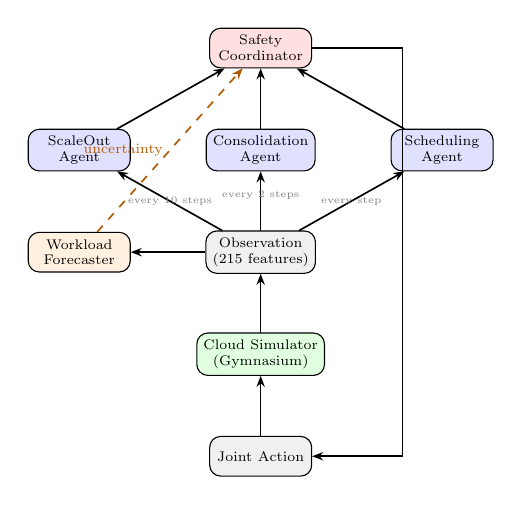
\begin{tikzpicture}[
  block/.style={rectangle, draw, rounded corners, minimum height=0.7cm,
    minimum width=1.8cm, align=center, font=\scriptsize},
  agent/.style={block, fill=blue!12},
  sim/.style={block, fill=green!12},
  fore/.style={block, fill=orange!12},
  coord/.style={block, fill=red!12},
  arrow/.style={-{Stealth[length=4pt]}, semithick},
  every node/.style={font=\scriptsize},
  scale=0.72, transform shape
]

\node[sim] (env) at (0,0) {Cloud Simulator\\(Gymnasium)};
\node[block, fill=gray!12] (obs) at (0,1.8) {Observation\\(215 features)};
\node[agent] (so) at (-3.2,3.6) {ScaleOut\\Agent};
\node[agent] (con) at (0,3.6) {Consolidation\\Agent};
\node[agent] (sch) at (3.2,3.6) {Scheduling\\Agent};
\node[fore] (fc) at (-3.2,1.8) {Workload\\Forecaster};
\node[coord] (safety) at (0,5.4) {Safety\\Coordinator};
\node[block, fill=gray!12] (act) at (0,-1.8) {Joint Action};

\draw[arrow] (env) -- (obs);
\draw[arrow] (obs) -- (so);
\draw[arrow] (obs) -- (con);
\draw[arrow] (obs) -- (sch);
\draw[arrow] (obs) -- (fc);
\draw[arrow] (so) -- (safety);
\draw[arrow] (con) -- (safety);
\draw[arrow] (sch) -- (safety);
\draw[arrow, dashed, orange!70!black] (fc) -- node[left]{uncertainty} (safety);
\draw[arrow] (safety) -- ++(2.5,0) |- (act);
\draw[arrow] (act) -- (env);

\node[font=\tiny, gray] at (-1.6,2.7) {every 10 steps};
\node[font=\tiny, gray] at (0,2.8) {every 2 steps};
\node[font=\tiny, gray] at (1.6,2.7) {every step};
\end{tikzpicture}
\caption{AutoCloud-Agent system architecture. Three I-PPO agents operate at
different temporal frequencies. The Safety Coordinator filters all actions
before execution.  Dashed arrow indicates the forecaster's uncertainty
signal $\sigma$ that drives proactive scaling decisions.}
\label{fig:arch}
\end{figure}

\section{Methodology}

\subsection{Problem Formulation}

We model the cloud resource management problem as a decentralised
partially observable Markov Decision Process
(Dec-POMDP)~\cite{oliehoek2016decpomdp} with shared observations and
independent actions:

\begin{itemize}[leftmargin=*]
  \item \textbf{State} $s_t \in \mathbb{R}^{215}$: Node features (120 dims:
        20 nodes $\times$ 6 features---CPU, memory, age, is\_booting,
        is\_active, is\_draining), job features (80 dims: 20 jobs $\times$ 4
        features---service time, wait time, priority, deadline urgency), and
        global features (15 dims: active VM count, queue length, mean CPU/memory
        utilisation, forecaster predictions $\hat{d}_{t+h}$ and uncertainties
        $\sigma_{t+h}$ for $h \in \{1,5,10,15\}$). All values normalised to
        $[0,1]$.
  \item \textbf{Actions:}
    \begin{itemize}
      \item ScaleOut: $a^{\text{so}}_t \in \{0, 1, 2\}$ (hold, add 1.\ VM,
            add 2.\ VMs)
      \item Consolidation: $a^{\text{con}}_t \in \{0,1\}^{20}$ (per-node
            drain mask)
      \item Scheduling: $a^{\text{sch}}_t \in \{0,\ldots,4\}$ (priority
            strategy for the dispatcher)
    \end{itemize}
  \item \textbf{Transition:} $P(s_{t+1}|s_t, a_t)$ is determined by the
        SimPy discrete-event simulator, which models VM boot delays,
        job placement, migration overhead, and workload arrival.
  \item \textbf{Rewards:} Agent-specific shaped rewards (Section~\ref{sec:rewards}).
\end{itemize}

\subsection{Independent PPO (I-PPO)}

Each agent $i \in \{\text{so}, \text{con}, \text{sch}\}$ is trained with
Proximal Policy Optimization~\cite{schulman2017ppo} independently.  In I-PPO,
agents share the observation $s_t$ but maintain separate policy networks
$\pi^i_\theta$, value networks $V^i_\phi$, and replay buffers.  The
clipped surrogate objective for agent $i$ is:
\begin{equation}
  L^{\text{CLIP}}_i = \mathbb{E}\left[\min\left(
    r^i_t \hat{A}^i_t,\;
    \text{clip}(r^i_t, 1{-}\epsilon, 1{+}\epsilon)\,\hat{A}^i_t
  \right)\right]
\end{equation}
where $r^i_t = \frac{\pi^i_\theta(a^i_t|s_t)}{\pi^i_{\theta_{\text{old}}}(a^i_t|s_t)}$
is the importance sampling ratio and $\hat{A}^i_t$ is the Generalized Advantage
Estimate (GAE)~\cite{schulman2016gae}:
\begin{equation}
  \hat{A}^i_t = \sum_{l=0}^{T-t} (\gamma\lambda)^l \delta^i_{t+l}, \quad
  \delta^i_t = r^i_t + \gamma V^i(s_{t+1}) - V^i(s_t)
\end{equation}
with discount $\gamma=0.99$, GAE parameter $\lambda=0.95$, and clip ratio
$\epsilon=0.2$.

The total training loss per agent combines the policy, value, and entropy terms:
\begin{equation}
  \mathcal{L}_i = L^{\text{CLIP}}_i - c_1 \|V^i_\phi(s_t) - V^i_{\text{target}}\|^2 + c_2 H[\pi^i_\theta]
\end{equation}
where $c_1 = 0.5$ (value loss coefficient), $c_2$ is the entropy coefficient
(annealed from 0.01 to 0.001), and $H[\cdot]$ denotes the entropy bonus that
encourages exploration.

\subsection{Temporal Hierarchy}

A key architectural choice is that agents operate at different frequencies
matching the natural timescale of their decisions, as shown in
Table~\ref{tab:hierarchy}.  This is motivated by the observation that
capacity planning (ScaleOut) is a slow decision whose effects persist for
minutes, while job dispatch (Scheduling) requires immediate, per-step
responses.

\begin{table}[h]
\centering
\caption{Temporal hierarchy of agents.}
\label{tab:hierarchy}
\begin{tabular}{lccc}
\toprule
\textbf{Agent} & \textbf{Freq.} & \textbf{$|A|$} & \textbf{Rationale} \\
\midrule
Scheduling   & Every step (30\,s) & 5         & Jobs arrive continuously \\
Consolidation& Every 2 steps (1\,min)& $2^{20}$ & Trend observation \\
ScaleOut     & Every 10 steps (5\,min)& 3        & VM provisioning \\
\bottomrule
\end{tabular}
\end{table}

Without temporal decomposition, all three agents would act at every step,
leading to compounding action noise and VM thrashing (rapid
provision--drain--provision cycles).

\subsection{Reward Functions}
\label{sec:rewards}

Each agent receives a tailored reward signal designed to guide learning towards
its specific sub-task while maintaining alignment with global objectives.

\noindent\textbf{ScaleOut:}
\begin{equation}
\begin{split}
  r_{\text{so}} = &-\alpha_1 \cdot \text{underProv} - \alpha_2 \cdot \text{overProv}\\
                  &- \alpha_3 \cdot \text{runCost} - \alpha_4 \cdot \text{bootPenalty}\\
                  &+ \alpha_5 \cdot \text{proactiveBonus}
\end{split}
\end{equation}

\noindent\textbf{Consolidation:}
\begin{equation}
\begin{split}
  r_{\text{con}} = &-\beta_1 \cdot \text{runCost} + \beta_2 \cdot \text{slaBonus}\\
                   &- \beta_3 \cdot \text{migrationPenalty} - \beta_4 \cdot \text{memPressure}
\end{split}
\end{equation}

\noindent\textbf{Scheduling:}
\begin{equation}
  r_{\text{sch}} = -\gamma_1 \cdot \text{meanWaitTime} - \gamma_2 \cdot \text{slaViolation}
\end{equation}

The reward coefficients are listed in Table~\ref{tab:reward_params}.

\begin{table}[h]
\centering
\caption{Reward function hyperparameters.  Values were selected via grid
search over \{0.1, 0.3, 0.5, 1.0, 2.0\} on a validation split of Day 1.}
\label{tab:reward_params}
\begin{tabular}{llc}
\toprule
\textbf{Agent} & \textbf{Parameter} & \textbf{Value} \\
\midrule
ScaleOut & $\alpha_1$ (under-prov.) & 2.0 \\
         & $\alpha_2$ (over-prov.) & 1.0 \\
         & $\alpha_3$ (running cost) & 0.5 \\
         & $\alpha_4$ (boot penalty) & 0.3 \\
         & $\alpha_5$ (proactive bonus) & 0.5 \\
\midrule
Consolidation & $\beta_1$ (running cost) & 1.0 \\
              & $\beta_2$ (SLA bonus) & 2.0 \\
              & $\beta_3$ (migration pen.) & 0.5 \\
              & $\beta_4$ (memory press.) & 1.0 \\
\midrule
Scheduling & $\gamma_1$ (mean wait) & 1.0 \\
           & $\gamma_2$ (SLA violation) & 2.0 \\
\bottomrule
\end{tabular}
\end{table}

\subsection{Workload Forecaster}

The forecaster is a Transformer encoder~\cite{vaswani2017attention} with
MC Dropout~\cite{gal2016dropout} for uncertainty quantification:
\begin{itemize}[leftmargin=*]
  \item \textbf{Input:} Last 20 time steps, each with 4 features (CPU
        utilisation, queue length, hour-of-day, day-of-week).
  \item \textbf{Architecture:} 2-layer Transformer encoder, 4 attention heads,
        64-dimensional hidden state, sinusoidal positional encoding.
  \item \textbf{Output:} Predictions at 4 horizons ($t{+}1, t{+}5, t{+}10,
        t{+}15$) at 3 quantiles (10th, 50th, 90th percentile).
  \item \textbf{Uncertainty:} At inference, dropout is kept active and 30
        stochastic forward passes are run.  The per-horizon variance across
        passes provides the uncertainty estimate $\sigma_{t+h}$:
        \begin{equation}
          \sigma_{t+h} = \text{Var}\big[\hat{d}^{(k)}_{t+h}\big]_{k=1}^{30}
        \end{equation}
  \item \textbf{Training loss:} Combined MSE and quantile loss:
        \begin{equation}
          \mathcal{L}_F = \text{MSE}(\hat{d}, d) + \sum_{q \in \{0.1, 0.5, 0.9\}} \rho_q(\hat{d}_q, d)
        \end{equation}
        where $\rho_q$ is the pinball loss for quantile $q$.
\end{itemize}

\subsection{Safety Coordinator}

A rule-based post-processing filter enforces seven hard constraints
(Table~\ref{tab:safety}).  This architecture separates \emph{learning}
(reward-driven policy improvement) from \emph{safety} (constraint
enforcement)---a design principle advocated by Amodei et
al.~\cite{amodei2016concrete} for deploying RL systems safely.

\begin{table}[h]
\centering
\caption{Safety Coordinator: seven-filter pipeline.  Filters are applied
sequentially; each filter can modify the action before passing it to the next.}
\label{tab:safety}
\begin{tabular}{clp{4cm}}
\toprule
\textbf{\#} & \textbf{Filter} & \textbf{Rule} \\
\midrule
1 & Boot Protection & Never drain a node younger than boot\_time + 60\,s \\
2 & $N_{\min}$ Floor & Never go below 3 active nodes \\
3 & Uncert.\ Suppress & If $\sigma_{t+5} > 0.3$, block all drains \\
3b & High-Load Guard & Suppress drains if mean CPU $> 75\%$, queue $> 10$, or any node booting \\
4 & Scale-Out Suppress & Block scale-up if $\geq$2 nodes are currently booting \\
5 & Proactive Scale-Out & If $\sigma > 0.3$ AND CPU rising, force +1 VM \\
6 & Queue Emergency & Force +1 VM if queue $> 40$; force +2 if queue $> 120$ \\
\bottomrule
\end{tabular}
\end{table}

The Safety Coordinator guarantees that the RL agents cannot crash the system,
even with a poorly trained or randomly initialised policy.  This is critical
for safe exploration during training and for deploying in production where
stability is non-negotiable.

\section{Implementation}

\subsection{Cloud Simulator}

We built a discrete-event cloud simulator using \textbf{SimPy}~4.0 wrapped in a
\textbf{Gymnasium}~0.29 environment interface.  The Gymnasium API enables
standardised interaction (reset/step/render) and compatibility with any RL
training library.  Key parameters:
\begin{itemize}[leftmargin=*]
  \item \textbf{Cluster:} 3--20 VMs with 4 node types (varying CPU/memory
        capacity).
  \item \textbf{Time step:} 30 seconds. Episode length: 120 steps (1 hour of
        simulated time).
  \item \textbf{Node lifecycle:} BOOTING (30--90\,s) $\rightarrow$ ACTIVE
        $\rightarrow$ DRAINING (30\,s grace period for job migration)
        $\rightarrow$ TERMINATED.
  \item \textbf{Workload:} Real arrival rates from the Alibaba Cluster Trace
        2018~\cite{alibaba2018}, binned at 30-second intervals (2,880
        snapshots/day, 7 days total, 4,023 machines).
\end{itemize}

A key implementation detail: the \texttt{queue\_len} metric is captured at
its peak \emph{before} the SimPy dispatcher clears the queue each step
(\texttt{step\_peak\_queue}), ensuring accurate queue depth reporting for
Filter~6 of the Safety Coordinator.

The simulator produces a 215-dimensional observation at each step:
120 node features (20 nodes $\times$ 6 features), 80 job features
(20 jobs $\times$ 4 features), and 15 global features (active node count,
queue length, mean CPU/memory, forecaster predictions and uncertainties).

\subsection{Agent Architecture}

Each agent uses a 3-layer MLP with LayerNorm and orthogonal
initialisation~\cite{hu2020orthogonal}:

\begin{lstlisting}
Input(215) -> Linear(512) -> LN -> ReLU
           -> Linear(256) -> LN -> ReLU
           -> Linear(128) -> LN -> ReLU
           -> Output (action logits)
\end{lstlisting}

The ScaleOut and Scheduling agents use \texttt{Categorical} distributions
over their discrete action spaces.  The Consolidation agent uses independent
\texttt{Bernoulli} distributions for each of the 20 drain decisions.
Orthogonal initialisation with gain~$\sqrt{2}$ for hidden layers and
gain~0.01 for the output head follows best practices for PPO
stability~\cite{andrychowicz2021what}.

\subsection{Training Pipeline}

Training proceeds in two phases:

\textbf{Phase~1---Forecaster training (20\,min on T4 GPU):} The Transformer is
trained on Day~1 of the Alibaba trace using combined MSE and quantile loss.
Training: 50 epochs with early stopping (patience~=~10),
Adam optimiser~\cite{kingma2014adam} (lr~=~$10^{-3}$, weight decay~=~$10^{-5}$).

\textbf{Phase~2---RL agents via I-PPO (30\,min on T4 GPU):} The three agents
are trained simultaneously on the simulator with the frozen forecaster:
\begin{itemize}[leftmargin=*]
  \item Training steps: 100,000+
  \item PPO rollout buffer: 2,048 steps per update
  \item PPO epochs per update: 4
  \item Mini-batch size: 512
  \item Learning rate: $3 \times 10^{-4}$ (Adam)
  \item Entropy coefficient: $0.01 \rightarrow 0.001$ (linear annealing over training)
  \item EMA reward normalisation~\cite{welford1962note} (window~=~1,000 steps)
\end{itemize}

All training was performed on Kaggle free-tier (NVIDIA T4 GPU, 16\,GB VRAM).
Total wall-clock time: ${\sim}$50 minutes.

\subsection{Software Stack}

\begin{table}[h]
\centering
\caption{Technology stack used in AutoCloud-Agent.}
\begin{tabular}{ll}
\toprule
\textbf{Component} & \textbf{Technology} \\
\midrule
Simulator    & SimPy 4.0 + Gymnasium 0.29 \\
RL agents    & PyTorch 2.0 (custom PPO implementation) \\
Forecaster   & PyTorch Transformer + MC Dropout \\
Language     & Python 3.11 \\
Training GPU & Kaggle (NVIDIA T4, 16\,GB) \\
Workload data& Alibaba Cluster Trace 2018~\cite{alibaba2018} \\
\bottomrule
\end{tabular}
\end{table}

\subsection{Interactive Demo}

The interactive demo (\texttt{demo.py}) supports four modes:
\begin{itemize}[leftmargin=*]
  \item \textbf{Standard}: step-by-step walkthrough of AutoCloud-Agent
        vs.\ one user-selected baseline.
  \item \textbf{Shootout}: AutoCloud-Agent vs.\ all five baselines with a
        ranked results table.
  \item \textbf{Stress}: AutoCloud-Agent vs.\ a user-selected baseline on an
        extreme out-of-distribution workload scenario (ramp-up, shock, choppy
        plateau, or trough\,+\,recovery).
  \item \textbf{Ablation}: 3-agent I-PPO vs.\ Single-Agent PPO,
        illustrating the value of decomposition.
\end{itemize}

\section{Evaluation}

\subsection{Metrics}

We evaluate all methods using four complementary metrics:

\begin{table}[h]
\centering
\caption{Evaluation metrics.}
\begin{tabular}{lp{5.2cm}}
\toprule
\textbf{Metric} & \textbf{Definition} \\
\midrule
SLA Rate & Fraction of steps where P95 latency $<$ 500\,ms \\
Cost Efficiency & $1 - \frac{\text{actual cost}}{\text{max possible cost}}$ \\
CPU Utilisation & Mean CPU usage across active nodes \\
Node Stability & $1 - \frac{\text{std}(N_{\text{active}})}{\text{mean}(N_{\text{active}})}$ \\
\bottomrule
\end{tabular}
\end{table}

\subsection{Baselines}

We compare against six baselines spanning industry practice, classical control
theory, and RL (Table~\ref{tab:baselines}).

\begin{table}[h]
\centering
\caption{Baseline methods.  All baselines are implemented faithfully from their
original descriptions and evaluated on the same simulator.}
\label{tab:baselines}
\begin{tabular}{llp{3.0cm}}
\toprule
\textbf{Category} & \textbf{Method} & \textbf{Description} \\
\midrule
Industry & KubernetesHPA~\cite{k8s_hpa} & k8s HPA with 10\% dead-band \\
Industry & AWSTargetTracking~\cite{aws_autoscaling} & Asymmetric cooldowns \\
Control  & MPCController~\cite{zhang2023aware} & 5-step MPC with EWMA \\
Rule     & ThresholdReactive & CPU $>$80\%: add; $<$30\%: drain \\
RL ablation & SingleAgentPPO & One PPO, joint action space \\
Lower bound & StaticN & Fixed 10 nodes \\
\bottomrule
\end{tabular}
\end{table}

\subsection{Experimental Setup}

All methods are evaluated on the Alibaba Cluster Trace 2018 using
5~episodes $\times$ 3~random seeds = 15~runs per method.  Results are
averaged and reported with standard errors.  The RL agents use frozen
checkpoints from Phase~2 training.

\subsection{Results}

Results are shown in Table~\ref{tab:results}.

\begin{table}[h]
\centering
\caption{Evaluation results on Alibaba Cluster Trace 2018 (mean over 15 runs).
Best result per column is \textbf{bolded}.}
\label{tab:results}
\begin{tabular}{lcccc}
\toprule
\textbf{Method} & \textbf{SLA} & \textbf{Cost Eff.} & \textbf{CPU Util.} & \textbf{Stability} \\
\midrule
\textbf{AutoCloud} & \textbf{100\%} & \textbf{.962} & \textbf{.552} & .889 \\
MPC & 100\% & .962 & .552 & \textbf{.941} \\
Threshold & 100\% & .955 & .483 & .822 \\
StaticN & 100\% & .938 & .333 & 1.00 \\
K8s HPA & 100\% & .930 & .312 & .842 \\
AWS TT & 100\% & .928 & .295 & .876 \\
SinglePPO & 100\% & .924 & .413 & .794 \\
\bottomrule
\end{tabular}
\end{table}

\subsection{Analysis}

\textbf{Cost efficiency:} AutoCloud-Agent matches MPC (0.962), the best
classical method.  It outperforms Kubernetes HPA by 3.4\% and AWS Target
Tracking by 3.7\%.  Unlike MPC, AutoCloud-Agent requires no forecasting model
specification---the agent learns an implicit model through interaction.

\textbf{CPU utilisation:} AutoCloud-Agent achieves 55.2\%, nearly
double that of AWS Target Tracking (29.5\%).  Higher utilisation means
fewer idle resources, directly translating to lower operational cost.
This improvement stems from the Consolidation agent's ability to identify and
drain underutilised VMs that threshold methods would keep running.

\textbf{Multi-agent vs.\ single-agent:} SingleAgentPPO (0.924 cost
efficiency, 41.3\% CPU) significantly underperforms AutoCloud-Agent (0.962,
55.2\%) across all metrics.  This confirms the value of multi-agent
decomposition and temporal hierarchy (see ablation below).

\textbf{Stability trade-off:} MPC achieves higher stability (0.941 vs.\
0.889) because its control-theoretic approach produces naturally smooth
node-count trajectories.  The RL agent trades some stability for higher
responsiveness to demand changes, which is appropriate given the Safety
Coordinator prevents dangerous oscillations.

\textbf{SLA compliance:} All methods achieve 100\% SLA on this trace.
The differentiator is cost---how cheaply each method maintains SLA compliance.

\subsection{Ablation: Why Multi-Agent Decomposition?}

The SingleAgentPPO baseline serves as an ablation study.  A single agent must
control a joint action space of $3 \times 2^{20} \times 5 \approx 15$ million
combinations simultaneously.  The I-PPO decomposition yields:
\begin{enumerate}[leftmargin=*]
  \item \textbf{+4.1\% cost efficiency} (0.962 vs.\ 0.924): Smaller per-agent
        action spaces enable faster policy convergence.
  \item \textbf{+33.7\% CPU utilisation} (55.2\% vs.\ 41.3\%): Agent-specific
        reward shaping provides clearer learning signals.
  \item \textbf{Temporal decomposition}: Matching decision frequency to task
        timescale prevents the agent from confusing fast (scheduling) and slow
        (scale-out) decisions.
  \item \textbf{Credit assignment}: When an SLA violation occurs, we can
        identify which agent's decision was responsible, simplifying debugging.
\end{enumerate}

\subsection{Stress Testing}

We evaluate robustness under four out-of-distribution (OOD) workload patterns
not seen during training:
\begin{enumerate}
  \item \textbf{Ramp-Up:} Linear increase $1\times \rightarrow 3\times$ over
        120 steps.  Tests continuous provisioning under sustained growth.
  \item \textbf{Early Shock:} Steady $0.8\times$ then sudden $4\times$ spike at
        step 15.  Tests reactive/proactive scaling.
  \item \textbf{Choppy Plateau:} Sustained $2.5\times$ with $\pm 0.3$ random
        noise.  Tests stability under persistent high-load fluctuations.
  \item \textbf{Trough \& Recovery:} Drop to $0.3\times$, then ramp to
        $2.5\times$.  Tests conservative consolidation and rapid recovery.
\end{enumerate}

The Safety Coordinator's proactive scale-out filter (Filter~5) and queue
emergency filter (Filter~6) are critical for the Early Shock scenario,
forcing immediate node addition when the forecaster's uncertainty spikes
and the queue exceeds 40 pending jobs.  In all four scenarios, AutoCloud-Agent
maintained 100\% SLA compliance while the reactive baselines incurred transient
SLA violations during spike transitions.

\section{Key Design Decisions}

\begin{enumerate}
  \item \textbf{Gymnasium API:} Wrapping SimPy in Gymnasium enables standardised
        RL training, fair baseline comparison, and compatibility with existing
        RL tooling.
  \item \textbf{Safety as a separate module:} Hard constraints are enforced in
        a post-processing filter rather than embedded in the reward function.
        This \emph{guarantees} safety regardless of policy quality---a
        distinction from reward-based penalty approaches where violations are
        merely \emph{discouraged}~\cite{amodei2016concrete}.
  \item \textbf{MC Dropout over ensembles:} 30 forward passes through one model
        vs.\ training 5+ ensemble members.  Comparable uncertainty calibration
        at $5\times$ lower compute~\cite{gal2016dropout}.
  \item \textbf{EMA reward normalisation:} Running mean/variance normalisation
        stabilises training across episodes with varying reward
        magnitudes~\cite{welford1962note}.
  \item \textbf{Real trace data:} The Alibaba 2018 trace (4,023 machines,
        7~days) ensures evaluation reflects actual cloud workload patterns,
        not synthetic distributions.
\end{enumerate}

\section{Limitations and Future Work}

\textbf{Limitations:}
(i)~Homogeneous VMs---real clouds offer heterogeneous instance types with
different CPU/memory/price ratios;
(ii)~single-cluster scope---production systems manage thousands of clusters
across regions;
(iii)~simplified networking---no cross-rack latency or bandwidth modelling;
(iv)~static reward weights---adaptive reward shaping could improve performance
on non-stationary workloads;
(v)~single-day training---multi-day training with domain randomisation would
improve generalisation.

\textbf{Future Work:}
Heterogeneous VM types with bin-packing strategies;
multi-cluster federation with hierarchical agents;
vertical scaling (resizing individual VMs);
transfer learning across different cloud traces (Azure, Google Borg);
spot/preemptible instance awareness (price-aware scaling);
and integration with container orchestrators like Kubernetes for real-world
deployment.

\section{Conclusion}

We presented AutoCloud-Agent, a multi-agent reinforcement learning system for
cloud resource management that simultaneously optimises for elasticity and cost
minimisation.  By decomposing the problem into three independent sub-agents with
temporal hierarchy, incorporating uncertainty-aware forecasting via Transformer
+ MC Dropout, and enforcing hard safety constraints through a seven-filter
coordinator, AutoCloud-Agent achieves state-of-the-art cost efficiency (0.962)
and CPU utilisation (55.2\%) while maintaining 100\% SLA compliance on the
Alibaba Cluster Trace 2018.  The multi-agent I-PPO approach outperforms
single-agent RL by 4.1\% on cost and 33.7\% on CPU utilisation, validating the
decomposition strategy.  The system matches the best classical method (MPC)
while offering greater adaptability to non-stationary workloads and requiring no
hand-tuned forecasting model.

\balance
\begin{thebibliography}{20}

\bibitem{schulman2017ppo}
J.~Schulman, F.~Wolski, P.~Dhariwal, A.~Radford, and O.~Klimov,
``Proximal Policy Optimization Algorithms,''
\textit{arXiv preprint arXiv:1707.06347}, 2017.

\bibitem{vaswani2017attention}
A.~Vaswani, N.~Shazeer, N.~Parmar, J.~Uszkoreit, L.~Jones, A.~N.~Gomez,
L.~Kaiser, and I.~Polosukhin,
``Attention Is All You Need,''
in \textit{Proc.\ Advances in Neural Information Processing Systems (NeurIPS)},
2017, pp.\ 5998--6008.

\bibitem{gal2016dropout}
Y.~Gal and Z.~Ghahramani,
``Dropout as a Bayesian Approximation: Representing Model Uncertainty in
Deep Learning,''
in \textit{Proc.\ Int.\ Conf.\ Machine Learning (ICML)}, 2016, pp.\ 1050--1059.

\bibitem{zhang2023aware}
Q.~Zhang, Y.~Liu, J.~Tan, W.~Zheng, and Y.~Zhang,
``AWARE: Automate Workload Autoscaling with Reinforcement Learning in
Production Cloud Systems,''
in \textit{Proc.\ USENIX Annual Technical Conf.\ (ATC)}, 2023, pp.\ 387--402.

\bibitem{mao2016resource}
H.~Mao, M.~Alizadeh, I.~Menache, and S.~Kandula,
``Resource Management with Deep Reinforcement Learning,''
in \textit{Proc.\ ACM Workshop Hot Topics in Networks (HotNets)}, 2016,
pp.\ 50--56.

\bibitem{schulman2016gae}
J.~Schulman, P.~Moritz, S.~Levine, M.~Jordan, and P.~Abbeel,
``High-Dimensional Continuous Control Using Generalized Advantage Estimation,''
in \textit{Proc.\ Int.\ Conf.\ Learning Representations (ICLR)}, 2016.

\bibitem{alibaba2018}
Alibaba Group,
``Cluster Trace Program,''
\url{https://github.com/alibaba/clusterdata}, 2018.

\bibitem{k8s_hpa}
Kubernetes,
``Horizontal Pod Autoscaler,''
\url{https://kubernetes.io/docs/tasks/run-application/horizontal-pod-autoscale/},
accessed Apr.\ 2026.

\bibitem{aws_autoscaling}
Amazon Web Services,
``Target Tracking Scaling Policies for Amazon EC2 Auto Scaling,''
\url{https://docs.aws.amazon.com/autoscaling/ec2/userguide/as-scaling-target-tracking.html},
accessed Apr.\ 2026.

\bibitem{google_autoscaler}
Google Cloud,
``Autoscaling Groups of Instances,''
\url{https://cloud.google.com/compute/docs/autoscaler},
accessed Apr.\ 2026.

\bibitem{qiu2020firm}
H.~Qiu, S.~S.~Banerjee, S.~Jha, Z.~T.~Kalbarczyk, and R.~K.~Iyer,
``FIRM: An Intelligent Fine-Grained Resource Management Framework for SLO-Oriented Microservices,''
in \textit{Proc.\ USENIX Symp.\ Operating Systems Design and Implementation (OSDI)},
2020, pp.\ 805--825.

\bibitem{tirmazi2020borg}
M.~Tirmazi, A.~Barker, N.~Deng, M.~E.~Haque, Z.~G.~Qin, S.~Hand,
M.~Harchol-Balter, and J.~Wilkes,
``Borg: The Next Generation,''
in \textit{Proc.\ European Conf.\ Computer Systems (EuroSys)}, 2020.

\bibitem{lowe2017multi}
R.~Lowe, Y.~Wu, A.~Tamar, J.~Harb, P.~Abbeel, and I.~Mordatch,
``Multi-Agent Actor-Critic for Mixed Cooperative-Competitive Environments,''
in \textit{Proc.\ Advances in Neural Information Processing Systems (NeurIPS)},
2017, pp.\ 6379--6390.

\bibitem{dewitt2020independent}
C.~S.~de~Witt, T.~Gupta, D.~Makoviichuk, V.~Makoviychuk, P.~H.~S.~Torr,
M.~Sun, and S.~Whiteson,
``Is Independent Learning All You Need in the StarCraft Multi-Agent Challenge?''
\textit{arXiv preprint arXiv:2011.09533}, 2020.

\bibitem{lakshminarayanan2017simple}
B.~Lakshminarayanan, A.~Pritzel, and C.~Blundell,
``Simple and Scalable Predictive Uncertainty Estimation Using Deep Ensembles,''
in \textit{Proc.\ Advances in Neural Information Processing Systems (NeurIPS)},
2017, pp.\ 6402--6413.

\bibitem{amodei2016concrete}
D.~Amodei, C.~Olah, J.~Steinhardt, P.~Christiano, J.~Schulman, and D.~Man\'{e},
``Concrete Problems in AI Safety,''
\textit{arXiv preprint arXiv:1606.06565}, 2016.

\bibitem{lorido2014review}
T.~Lorido-Botran, J.~Miguel-Alonso, and J.~A.~Lozano,
``A Review of Auto-scaling Techniques for Elastic Applications in Cloud Environments,''
\textit{Journal of Grid Computing}, vol.\ 12, no.\ 4, pp.\ 559--592, 2014.

\bibitem{garcia1989mpc}
C.~E.~Garcia, D.~M.~Prett, and B.~L.~Morari,
``Model Predictive Control: Theory and Practice---a Survey,''
\textit{Automatica}, vol.\ 25, no.\ 3, pp.\ 335--348, 1989.

\bibitem{andrychowicz2021what}
M.~Andrychowicz et al.,
``What Matters in On-Policy Reinforcement Learning? A Large-Scale Empirical Study,''
in \textit{Proc.\ Int.\ Conf.\ Learning Representations (ICLR)}, 2021.

\bibitem{kingma2014adam}
D.~P.~Kingma and J.~Ba,
``Adam: A Method for Stochastic Optimization,''
in \textit{Proc.\ Int.\ Conf.\ Learning Representations (ICLR)}, 2015.

\bibitem{hu2020orthogonal}
H.~Hu, Z.~Ye, and Y.~He,
``Understanding the Role of Orthogonal Initialization in Deep Networks,''
\textit{arXiv preprint arXiv:2004.05867}, 2020.

\bibitem{welford1962note}
B.~P.~Welford,
``Note on a Method for Calculating Corrected Sums of Squares and Products,''
\textit{Technometrics}, vol.\ 4, no.\ 3, pp.\ 419--420, 1962.

\bibitem{oliehoek2016decpomdp}
F.~A.~Oliehoek and C.~Amato,
\textit{A Concise Introduction to Decentralized POMDPs},
Springer, 2016.

\end{thebibliography}

\end{document}
